\documentclass{article}
\usepackage[letterpaper,body={6.1in,9in},top=.8in,left=1.2in]{geometry}
\usepackage[no-math]{fontspec}
\usepackage{verbatim,fancyvrb}
\usepackage{gretl}
%\usepackage{amsmath}
\usepackage{graphicx}
\usepackage[authoryear]{natbib}
\usepackage{hyperref}

\setmonofont{DejaVu Sans Mono}[Scale=0.9]

\setlength{\parindent}{0pt}
\setlength{\parskip}{1ex}

\hypersetup{pdftitle={Holt 2.0},
            pdfauthor={Ignacio Díaz-Emparanza and Allin Cottrell},
            colorlinks=true,
            linkcolor=blue,
            urlcolor=red,
            citecolor=steel,
            bookmarksnumbered=true,
            plainpages=false
}

\begin{document}

\begin{center}
  {\Large \textbf{Holt 2.0}} \\[6pt]
  Ignacio Díaz-Emparanza and Allin Cottrell \\[6pt]
  2026-09-14
\end{center}

\section{Introduction}
\label{sec:intro}

This package implements the forecasting method devised by C. C. Holt
\citeyearpar{holt57}, namely double exponential smoothing with level and
trend and components.  It requires time-series data. If you want triple
exponential smoothing (with a seasonal component), as in
\citealt{winters60}), try the \textsf{Winters} package.

A prior version of this package (1.0) was written by Ignacio
Díaz-Emparanza in 2015. This revision was written by Allin Cottrell,
exploiting modern hansl syntax and adding functionality for automatic
determination of the Holt smoothing parameters. See
Section~\ref{sec:update} below for help with updating scripts for use
with version 2.

The filtering recursions and forecasting equation for Holt's method are
shown below. The notation is based on \cite[section 8.2]{hyndman2021}:
$\ell$ denotes the level and $b$ the trend or slope; $\alpha$ and
$\beta$ are the smoothing parameters.

\begin{align*}
  \ell_t &= \alpha y_t + (1-\alpha) (\ell_{t-1} + b_{t-1})\\
  b_t &= \beta (\ell_t - \ell_{t-1}) + (1-\beta) b_{t-1}\\
  \hat{y}_{t+h|t} &= \ell_t + hb_t
\end{align*}

Like most functions in gretl, \texttt{Holt} confines its operations
to the sample range in force when the function is called. We'll refer
to the (1-based) start and end of this range as $t_1$ and $t_2$,
respectively.\footnote{This range can be set via the \texttt{smpl}
  command. If \texttt{smpl} has not been invoked since a dataset was
  opened $t_1$ will equal 1 and $t_2$ will equal the total number of
  observations.}  In addition, let $T$ denote the date of the last
valid observation of the variable to be predicted, $y$.

There are two cases to be considered:
\begin{enumerate}
\item $T < t_2$: in this case there's a `tail' of observations for
  which values of $y_t$ are not available.  \texttt{Winters} will by
  default produce predictions for these observations.
\item $T = t_2$: there's no tail for genuine out-of-sample prediction,
  but you can specify a number of observations, \texttt{ntest}, to
  reserve for pseudo-out-of-sample prediction. In that case the
  Holt training recursion will be terminated at observation $T-$
  \texttt{ntest}.
\end{enumerate}

If you want case 1 but your dataset doesn't contain any extra trailing
observations it's straightforward to add them using the
\texttt{dataset addobs} command, or via the \textsf{Add observations}
item under the \textsf{Data} menu in the graphical interface.

Conversely, if the dataset does contain extra trailing observations
but you want case 2, specifying a positive value for \texttt{ntest}
will result in the extra observations being ignored and
pseudo-out-of-sample forecasts being produced.

\section{The public functions}

The primary function has the following signature:
\begin{nscode}
function bundle Holt (const series y, const bundle specs[null])
\end{nscode}

The required argument \texttt{y} specifies the series to be processed.
The second argument---which can be omitted, as indicated by the
\texttt{null} modifier---may contain one or more of the following
options:

\begin{itemize}
\item \texttt{theta} (matrix): if supplied, this must be a 2-vector
  holding the smoothing parameters $\theta$ = ($\alpha$, $\beta$), with
  each parameter in $[0,1]$. If \texttt{parms} is not given these
  parameters are determined automatically.
\item \texttt{ntest} (integer): specifies the number of
  observations at the end of the range of \texttt{y} values to reserve
  for testing via pseudo-out-of-sample forecasting. The default value
  is 0.
\item \texttt{verbose} (integer): controls the verbosity of output, with
  levels 0, 1 (the default), 2 or 3.
\end{itemize}

The return value from \texttt{Holt} is is a bundle containing the
following elements:
\begin{itemize}
\item \texttt{theta}: a 2-vector holding the smoothing parameter
  values.
\item \texttt{init}: a 2-vector of holding the initializer: level and
  trend.
\item \texttt{ntest}: a non-negative integer indicating how many
  observations were reserved for pseudo-out-of-sample forecasting.
\item \texttt{W}: a $T \times 4$ matrix.  Column 1 holds the data passed
  as \texttt{y}; columns 2 and 3 hold the estimated level and trend; and
  column 4 holds forecasts. More details on this matrix are provided
  below.
\item \dtk{RMSE_train}: the root mean squared error for the 1-step
  ahead forecasts made using the training data.
\end{itemize}
If \texttt{ntest} is non-zero, two additional items will be included
in the bundle, namely the RMSE and Mean Absolute Error for the
pseudo-out-of-sample forecasts, under the keys \dtk{RMSE_test} and
\dtk{MAE_test}.

A simple plotting function is also supplied:
\begin{nscode}
function void Holt_plot (bundle *b, int ptype)
\end{nscode}
The first argument should be a bundle obtained from \texttt{Holt} and
the second argument should be either 1 for a plot of actual and forecast
values, or 2 for a three-part plot of the level, trend and irregular
components.

\section{Command-line usage}
\label{sec:auto}

We'll start with a simple example: replication of the Australian
population example given in \cite[section[8.2]{hyndman2021}. Here's the
hansl code:\label{pg:ex1}
\begin{nscode}
open auspop.gdt --frompkg=Holt
dataset addobs 10
bundle hb = Holt(pop)
\end{nscode}

The \texttt{auspop} dataset contains 58 annual observations from
1960 to 2017, which will be used for training the model. The ten
added observations, 2018 to 2027, will then be used for
out-of-sample forecasting. Since \texttt{theta} is not not specified
both the parameters and the initializer for the Holt recursion
will be optimized automatically; see section~\ref{sec:details} for
details.

One might choose, instead, to use the \texttt{ntest} option to get
\texttt{Holt} to generate eight pseudo-out-of-sample forecasts:
\begin{nscode}
open auspop.gdt --frompkg=Holt
bundle hb = Holt(pop, _(ntest=8))
\end{nscode}
This will produce forecasts for 2010 to 2017.

\section{Output details}
\label{sec:out}

Table~\ref{tab:verbose} shows what is printed by \texttt{Holt} as a
function of the \texttt{verbose} option. An example of the table of
results displayed when \texttt{verbose} is 1 or greater is presented
in the lower part of listing~\ref{list:results}. The matrix \texttt{H}
that's included in the bundle returned by \texttt{Holt} is
basically a matrix version of this table. If you want to grab the
columns of \texttt{H} as a list of series you can do something like
\begin{nscode}
bundle hb = Holt(pop)
list L = mat2list(hb.H)
list L print # show all the series in L
\end{nscode}

\begin{table}[htbp]
  \caption{Effect of the verbose option}
  \label{tab:verbose}
  \begin{tabular}{cp{4.5in}}
    \textit{verbose} & \textit{cumulative effect} \\[6pt]
    0 & Nothing is printed. \\
    1 & Parameters and initializer are reported, also a table
        of results (see below) and the SSE and RMSE for the
        training data.\\
    2 & If optimization is performed, partial information on
        progress of the iterative procedure is shown. \\
    3 & If optimization is performed, progress of the
        optimizer is shown in full.
  \end{tabular}
\end{table}

\begin{script}[htbp]
  \caption{Partial listing of results from the first example on
    page~\ref{pg:ex1}: Forecasts for 2018 and beyond are
    out-of-sample.}
  \label{list:results}
\begin{code}
Holt double exponential smoothing
Recursion runs from 1998:1 to 2017:4
Out-of-sample forecast: 2018:1 to 2020:4

automatic parameter values:
  α = 0.246679, β = 0.122927, γ = 0

estimated initializer:

level       9.7602
trend    -0.028109

traning SSE = 13.4951, RMSE = 0.410718

                  y        level        trend       season     forecast

1998:1     11.80604      9.79856     -0.01994     1.180433     11.48812
1998:2      9.27566      9.69731     -0.02994     0.981654      9.59922
1998:3      8.64249      9.54811     -0.04460     0.941049      9.09748
1998:4      9.29952      9.55357     -0.03844     0.958077      9.10509
...
2017:1     12.40642     10.63437      0.08623     1.180433     12.60120
2017:2     10.47120     10.70735      0.08460     0.981654     10.52392
2017:3     10.49917     10.88197      0.09567     0.941049     10.15576
2017:4     11.21082     11.15617    0.1176140     0.958077     10.51742
2018:1                                                         13.30794
2018:2                                                         11.18241
2018:3                                                         10.83055
2018:4                                                         11.13920
...
\end{code}
\end{script}

\section{GUI usage}
\label{sec:gui}

When you install this package you should get the option of attaching it
as the menu item \textsf{Variable/Filter} in gretl's main
window. Clicking this item brings up the dialog box shown in
Figure~\ref{fig:dialog}.

\begin{figure}[htpb]
  \centering
  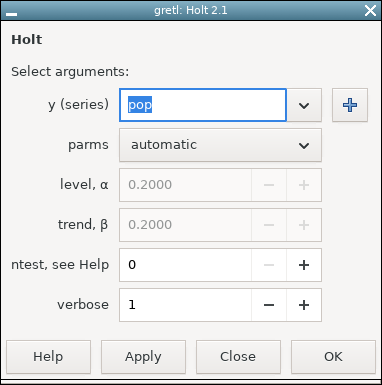
\includegraphics[scale=0.60]{Holt_dialog}
  \caption{Holt dialog, under the Variable/Filter menu}
  \label{fig:dialog}
\end{figure}

\begin{figure}[p]
  \centering
  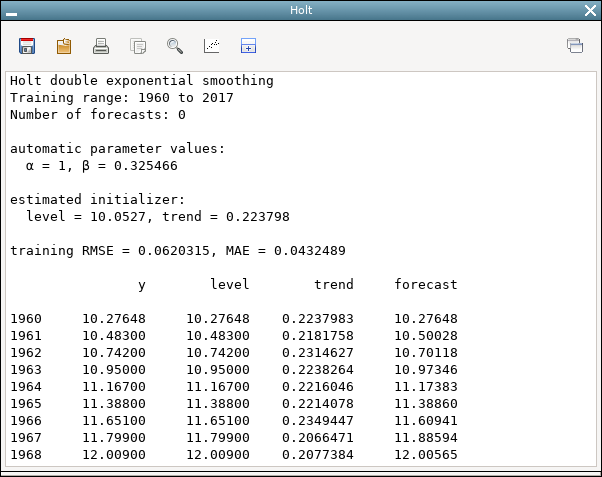
\includegraphics[scale=0.60]{output_window}
  \caption{Holt output window}
  \label{fig:output}
\end{figure}

Hopefully the choices available in the dialog are fairly
self-explanatory, but clicking the \textsf{Help} button will bring up a
brief explanation of each control. On clicking \textsf{OK} you should
get a window showing the results (Figure~\ref{fig:output}). The toolbar
at the top of this window includes a \textsf{Graph} button which gives
access to two types of plot, one showing actual and forecast \texttt{y}
and one showing the level, trend and irregular components.

\section{Technical details}
\label{sec:details}

This section offers some details on the rule-of-thumb initialization
with which the Holt recursion is started, and the optimization that
is carried out if \texttt{theta} is not given by the caller.

First, the rule-of-thumb is calculated as follows (where $\tau$ denotes
the first period in which $y$ is observed).
\begin{itemize}
\item The initial trend, $b_{\tau-1}$, is set to the first observed
  difference, $y_{\tau+1} - y_{\tau}$.
\item The initial level, $\ell_{\tau-1}$, is set to the first observed
  value minus the initial trend, $y_{\tau}-b_{\tau-1}$.
\end{itemize}

As regards optimization, two cases arise.
\begin{itemize}
\item If \texttt{theta} is not specified, the parameter values and
  initializer are optimized jointly, with the criterion of minimizing
  the sum of squared forecast errors for the training range. The
  starting point for the parameters is $\alpha = \beta = 0.2$; the
  starting point for the initializer is as described above. Optimization
  is performed using the L-BFGS algorithm (see the chapter on Numerical
  methods in the \GUG\ for details), with $\alpha$ and $\beta$
  constrained to lie in $[0,1]$.
\item If \texttt{theta} is given, the initializer is just the
  rule-of-thumb value; no optimization is performed. In principle the
  initializer could be optimized conditional on $\theta$ and that's a
  possible future refinement if it seems there's a real use case.
\end{itemize}

\section{Updating from Holt 1.0}
\label{sec:update}

Listing~\ref{list:compat} shows three cases drawing on the sample
script for version 1.0 of the package along with the revised code
required to produce similar results from version 2.0. Note that while
in version 1.0 the \texttt{Holt} arguments are strictly positional,
in version 2.0 they are in effect named, since they appear as elements
of a gretl bundle (apart from the first required series argument). And
the meaning of ``default smoothing parameters'' has changed: in
version 1.1 that means using a fixed parameter vector, FIXME
$\theta = (0.3, 0.1)$, while in version 2.0 it means that the
parameters are automatically optimized, along with the initializer.

When $\theta$ is specified the two versions should produce identical
forecasts: over the training range, $\hat{y}_{t|t-1}$, and over the
testing or out-of-sample range, $\hat{y}_{T+h|T}$ where $T$ is the last
training observation and $h = 1,2,\dots$.\footnote{FIXME. With one
  qualification: following Hyndman's procedure the first training
  forecast in version 2.0 is for the first observation of \texttt{y},
  while in version 1.0 the forecasts start $m$ periods later.}  So in
Case 1 we find that the testing results are the same for the two
versions, namely RMSE = XXX and MAE = XXX.

In Case 2 of the listing we could have had version 2.0 replicate the
results using the default $\theta$ from version 1.0, but it's more
informative to compare that default with optimized results. The
automatic $\theta$ in version 1.0 gives a slight improvement over Case
1: RMSE = XXX, MAE = XXX. The optimized parameters with 2.0 give
a more substantial improvement: RMSE = XXX, MAE = XXX.

In Case 3, with automatic parameters and genuine out-of-sample
forecasts, the forecasts will differ by version but we're obviously
not in a position to offer forecast evaluation statistics.

\begin{script}[p]
  \caption{Winters 1.1 examples with corresponding 2.0 code}
  \label{list:compat}
$\quad$ \\[1ex]
Common initial code
\begin{scode}
include Holt.gfn
open data9-3.gdt
\end{scode}
Case 1: Multiplicative, 4 testing forecasts, specified parameters
\begin{scode}
# version 1.1
bundle BW1 = Holt(reskwh, 1, 0.5, 0.1, 0.7, 4)
series reskwh_W_mul = BW.reskwh_W_mul

# version 2.0
bundle BW1 = Holt(reskwh, _(theta = {0.5, 0.1, 0.7}, ntest = 4))
series reskwh_W_mul = BW.W[,5]
\end{scode}
Case 2: Multiplicative, 4 testing forecasts, automatic parameters
\begin{scode}
# version 1.1
bundle BW2 = Holt(reskwh,1,,,,4)
series reskwh_W_mul = BW2.reskwh_W_mul

# version 2.0
bundle BW2 = Holt(reskwh, _(ntest=4))
series reskwh_W_mul = BW2.W[,5]
\end{scode}
Case 3: Additive, 4 out-of-sample forecasts, automatic parameters
\begin{scode}
# version 1.1
dataset addobs 4
bundle BW3 = Holt(reskwh, 0)
series reskwh_W_add = BW3.reskwh_W_add

# version 2.0
dataset addobs 4
bundle BW3 = Holt(reskwh, _(additive=1))
series reskwh_W_add = BW3.W[,5]
\end{scode}
\end{script}

The output data in the returned bundle also differ slightly across the
versions of the package. In version 1.0 four series are included: the
original series, the one-step ahead forecast, level-plus-trend, and
seasonal. Version 2.0 gives a four-column matrix holding the original
series, level, trend and forecast as in \cite{hyndman2021}.

\section{Change log}
\label{sec:log}

\begin{itemize}
\item \texttt{v2.0}: Initial release of substantially modified version.
\end{itemize}

\bibliographystyle{gretl}
\bibliography{gretl}

\end{document}
